%% ----------------------------------------------------------------
%% Methodology.tex
%% ---------------------------------------------------------------- 
\chapter{Methodology}
\section{Overview}

\begin{figure}[t]
\centering
\resizebox{0.98\linewidth}{!}{
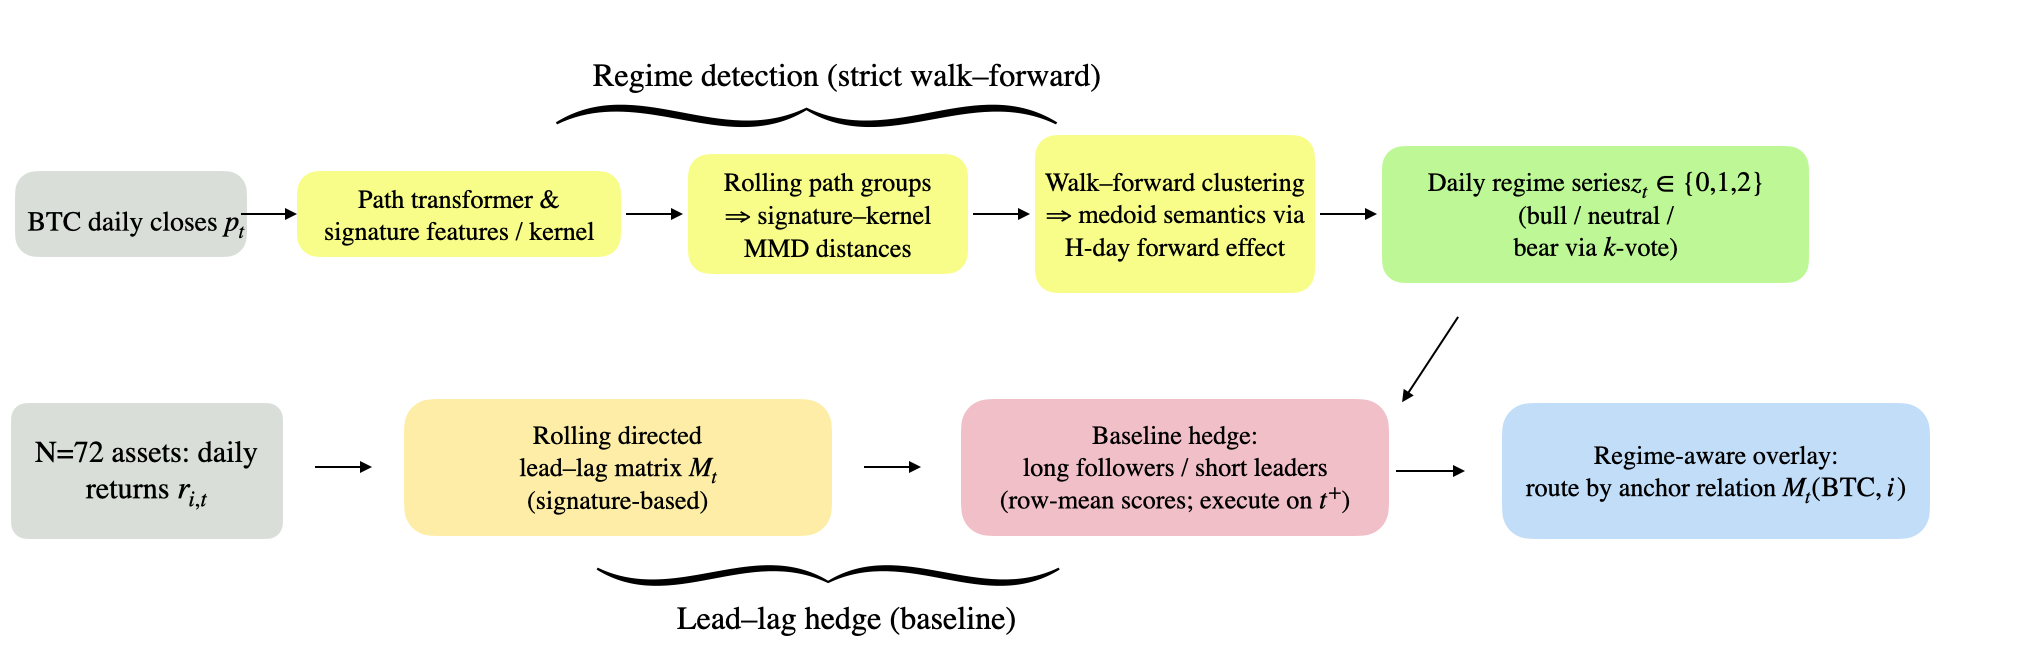
\includegraphics[]{process_plot/process.png}}
\caption{BTC-regime-aware lead-lag pipeline}
\end{figure}

This chapter presents an end-to-end pipeline. The pipeline links path-wise feature extraction, walk-forward regime detection, portfolio construction, and performance evaluation. We start from daily BTC closes. We then compute signature-based features that preserve temporal ordering, detect market regimes in a strictly leakage-free manner and finally use these regimes to condition a cross-sectional lead--lag hedge. All signals that we generate on day $t$ are executed on the next trading day $t^+$. All evaluations follow a unified daily calendar.

First, we extract \emph{path-wise} information with signature methods. We work with signature features or the signature kernel. These tools capture both the magnitude of price moves and the order of increments. This choice yields a representation that goes beyond scale-based indicators such as volatility. This representation encodes the geometry of the path.

Second, we run \emph{walk-forward clustering} on rolling path groups to obtain bull, neutral, and bear labels. At each decision date, our clustering uses only eligible historical groups whose forward windows are fully observed. Our mapping assigns clusters to economic states by their mean $H$-day forward returns. Our voting rule converts group-time labels into a daily series via a rolling vote. This procedure estimates semantics strictly from the past and avoids look-ahead.

Third, we form a baseline \emph{lead--lag} hedge and we overlay regime information. The baseline computes a rolling, directed lead--lag matrix from daily returns, and then forms an equal-weight long--short portfolio that is \emph{long followers} and \emph{short leaders}. The regime-aware overlay preserves this hedge structure. The overlay \emph{routes} constituents by the signed relation to a BTC anchor. In bull states, the overlay places co-moving assets on the long side and anti-moving assets on the short side. In bear states, the overlay flips the assignment. In neutral states, the overlay scales its effect by a fixed factor while keeping the hedge intact.

Finally, we evaluate both the baseline and the regime-aware strategies under a common protocol. We also report Sharpe and Sortino ratios, annualised volatility, cumulative return, and maximum drawdown. We finally analyse transaction-cost sensitivity separately. 




\section{Regime Detection}\label{sec:regime-detection}

\subsection{Data and Pre-processing}
This study constructs a daily market regime label $z_t\in\{0,1,2\}$, where $0=$ bear, $1=$ neutral, and $2=$ bull. The label is built from the anchor asset BTC from January 1, 2021 to June 30, 2024. The construction relies on path-wise statistics based on the signature kernel. Accordingly, the signal remains purely backward-looking at each date. The downstream portfolio module later uses this signal to modulate weights (Section~\ref{sec:regime}).

The notation defines $p_\tau$ as the BTC close price at time $\tau$ on a daily calendar. The time series is embedded as a path $\gamma=\{(\tau,p_\tau)\}_\tau$. The methodology operates on rolling \emph{subpaths} of fixed length. All timestamps are aligned to a unified timezone. Timestamps are also deduplicated before segmentation.

\subsection{Path Segmentation and Transformation}\label{sec:regime:seg}
The configuration fixes integers $n_{\text{steps}}\ge 2$ and $n_{\text{paths}}\ge 2$ and an overlap offset $o\ge 0$. The procedure slices $\gamma$ into consecutive subpaths of length $n_{\text{steps}}$ with stride $(n_{\text{steps}}-o)$:
\[
\textstyle
\mathrm{sub\_paths}
=\big\{\gamma^{(k)}\big\}_{k=1}^{N},\qquad
\gamma^{(k)}=\big((\tau_{k,1},p_{k,1}),\ldots,(\tau_{k,n_{\text{steps}}},p_{k,n_{\text{steps}}})\big).
\]
Next, the method collects \emph{groups} of $n_{\text{paths}}$ consecutive subpaths for two-sample comparisons:
\[
\textstyle
\mathrm{groups}=\big\{G_g\big\}_{g=1}^{G},\quad
G_g=\big(\gamma^{(g)},\gamma^{(g+1)},\ldots,\gamma^{(g+n_{\text{paths}}-1)}\big),
\]
so that each group $G_g$ covers a calendar span
$[s_g,e_g]=[\tau_{g,1},\,\tau_{g+n_{\text{paths}}-1,n_{\text{steps}}}]$.

Before computing similarities, a \emph{path transformer} \(T\) standardises levels to the initial value and normalises time:
\[
\widehat\gamma=T(\gamma);\quad
T=\text{(standardise\_path, time\_normalisation)}.
\]
For clarity, the baseline disables other transforms. The exclusions cover differences, cumulants, lead--lag lifts, and invisibility.

For each subpath $\gamma^{(k)}=((\tau_{k,1},p_{k,1}),\dots,(\tau_{k,n_{\text{steps}}},p_{k,n_{\text{steps}}}))$, the transformer applies level standardisation and time normalisation:
\[
\tilde p_{k,j}\;=\;\frac{p_{k,j}}{p_{k,1}},\qquad
\tilde \tau_{k,j}\;=\;\frac{j-1}{\,n_{\text{steps}}-1\,},\quad j=1,\dots, n_{\text{steps}}.
\]
Thus, the transformed subpath $\widehat\gamma^{(k)}=\{(\tilde\tau_{k,j},\tilde p_{k,j})\}_{j=1}^{n_{\text{steps}}}$ starts at level $1$ and lives on $[0,1]$.

\subsection{Signature--Kernel MMD Distance}\label{sec:regime:mmd}
The representation uses the path signature, a sequence of iterated integrals that encodes time ordering. The design avoids explicit truncation and explicit coordinates. Instead, the approach employs the \emph{signature kernel} $K_\Sigma$, which provides an implicit feature map $\Phi(\cdot)$ on path space. Consequently, the kernel enables two-sample testing and clustering without manual feature design~\cite{chevyrev2025primersignaturemethodmachine}.

The implementation instantiates $K_\Sigma$ via \texttt{higherOrderKME.sigkernel} with an ambient RBF on $(\text{time},\text{level})$. The settings use bandwidth $\sigma=1$, dyadic order $d=2$, and regularisation $\lambda=1$~\cite{salvi2021higher}. In turn, this configuration yields \emph{order-aware} similarities that suit regime discrimination.

The comparison between two groups of paths $G_g$ and $G_h$ uses maximum mean discrepancy (MMD) under $K_\Sigma$. The analysis denotes the implicit feature map by $\Phi(\cdot)$. The unbiased MMD$^2$ between bags of paths $A=\{x_a\}$ and $B=\{y_b\}$ is
\[
\mathrm{MMD}^2(A,B)
= \frac{1}{|A|(|A|-1)}\!\!\sum_{\substack{a\neq a'}}\! K_\Sigma(x_a,x_{a'})
+ \frac{1}{|B|(|B|-1)}\!\!\sum_{\substack{b\neq b'}}\! K_\Sigma(y_b,y_{b'})
- \frac{2}{|A||B|}\sum_{a,b} K_\Sigma(x_a,y_b).
\]
Accordingly, the procedure defines a symmetric \emph{group distance} as $D_{g,h}=\mathrm{MMD}(G_g,G_h)$. The system computes and stores the full precomputed distance matrix $D\in\mathbb{R}^{G\times G}$ for each $(n_{\text{steps}},n_{\text{paths}})$ configuration.

\begin{algorithm}[H]
\caption{Walk--forward regime detection (signature kernel)}
\label{alg:wf_regime_simple2e}
\Input{BTC daily closes $p_t$ on a unified calendar (2021-01-01 to 2024-06-30)}
\Params{Segmentation $(n_{\text{steps}}, n_{\text{paths}}, o{=}0)$; signature kernel $K_\Sigma$ (RBF, $\sigma{=}1$, dyadic order $2$, $\lambda{=}1$); WF window $w{=}30$ (groups); forward horizon $H{=}30$ (days); clusters $n_c{=}3$; thresholds $(\tau_+,\tau_-){=}(0,0)$; daily vote $k{=}7$}
\Output{Group labels $\mathrm{dir\_label}_g\in\{0,1,2\}$ and daily regimes $z_t\in\{0,1,2\}$}

\textbf{Segment \& transform}:
slice the path into subpaths of length $n_{\text{steps}}$, stack $n_{\text{paths}}$ to form groups $G_g$ with spans $[s_g,e_g]$; standardise level and normalise time

\textbf{Distances}:
compute precomputed $D$ with $D_{g,h}=\mathrm{MMD}(G_g,G_h)$ under $K_\Sigma$; clean $D$ (diag=0, symmetrise, fix NaN/Inf, clamp $<0$ to 0)

\For{$g \gets w-1$ \KwTo $G-1$}{
  \textbf{Eligible history} $E_g \leftarrow \{u\in[g-w+1,\,g-1]\ \mid$ the $H$-day forward return after $e_u$ is fully observed by just after $e_g\}$; if $|E_g|<n_c$, continue

  \textbf{Cluster \& prototypes}:
  run Agglomerative (complete, precomputed) on $D[E_g,E_g]$ to get $n_c$ clusters; for each cluster $c$, take medoid $m_c$ (min row-sum distance) and its forward effect $\mu_c$

  \textbf{Semantic mapping}:
  set $\psi(c){=}2$ if $\mu_c>\tau_+$ (bull); $\psi(c){=}0$ if $\mu_c<\tau_-$ (bear); otherwise $\psi(c){=}1$ (neutral)

  \textbf{Label current group}:
  assign $G_g$ to nearest medoid by $D$; let $c^\star$ be its cluster; set $\mathrm{dir\_label}_g \gets \psi(c^\star)$
}

\textbf{Daily series}:
for each day $t$, set $z_t$ to the majority label among the last $k$ completed groups ($e_u\le t$), breaking ties by recency; optionally merge consecutive equal labels for plotting
\end{algorithm}

Overall, grouping $n_{\text{paths}}$ consecutive subpaths forms two short bags of recent behaviour. The unbiased MMD on $K_\Sigma$ then serves as a path-wise two-sample distance between historical windows. Consequently, the distance highlights persistent geometric changes rather than pointwise volatility alone.

\subsection{Strict Walk--Forward Retraining and Labeling}\label{sec:wfstrict}
The calendar span of group $G_g$ is $[s_g,e_g]$. The historical window length is $w=\mathbf{30}$ groups, and the forward horizon is $H=\mathbf{30}$ trading days. The loop iterates for $g=w\!-\!1,\ldots,G\!-\!1$:

\begin{enumerate}[leftmargin=1.2em,itemsep=2pt,topsep=2pt]
\item \textbf{Eligibility (visibility constraint).}
The engine computes forward log returns $r^{(H)}_u$ for all groups $u$ using bars strictly after each group’s end time (``\texttt{start\_from=next}''). At decision $g$, the training set includes only those historical groups in $\{g-w+1,\ldots,g\}$ whose $H$-day future is fully observed by just after $e_g$. The current group $g$ is excluded from training.

\item \textbf{Clustering on eligible history.}
The clustering step runs Agglomerative Clustering (complete linkage, precomputed distances) on the eligible submatrix. The procedure yields $n_c=\mathbf{3}$ clusters. The prototype step computes each cluster’s \emph{medoid} as the member with the smallest row-sum distance.

\item \textbf{Semantic mapping (per-step).}
The scoring step uses the eligible groups’ forward returns $\{r^{(H)}_u\}$. The procedure requires \textbf{min\_count}$=\mathbf{10}$ eligible samples. The mapping assigns label $0$ (bear) to the cluster with the lowest mean if its effect $<\tau_{-}$. The mapping assigns label $2$ (bull) to the cluster with the highest mean if its effect $>\tau_{+}$. The thresholds are $(\tau_{+},\tau_{-})=(\mathbf{0},\mathbf{0})$. All remaining clusters receive label $1$ (neutral). No label is forced if thresholds are unmet.

\item \textbf{Label the current group only.}
The assignment step maps $G_g$ to the nearest medoid by $D$. The selected cluster is denoted $c^\star$. The algorithm sets $\mathrm{dir\_label}_g\in\{0,1,2\}$ to the semantic label of $c^\star$. Earlier groups remain unchanged.
\end{enumerate}

This loop re-estimates mappings strictly from history at every $g$. Consequently, the semantics adapt over time without leakage.

\subsection{Daily Regime Series via Rolling Vote}\label{sec:dailyvote}
Group labels live on irregular end times $\{e_g\}$. A majority vote produces a daily series $z_t$ using the last $k=\mathbf{7}$ \emph{completed} groups at each day $t$. A tie-breaking rule resolves ties by recency. A post-processing step merges consecutive days with the same label into non-overlapping spans for visualisation. An exported date-indexed daily series (values $0/1/2$) then supports backtesting.


\section{Lead--Lag Dependence}\label{sec:leadlag}

\begin{algorithm}[H]
\caption{Rolling signature--based lead--lag matrix}
\label{alg:sig_leadlag_2e}
\Input{Daily log returns $r_{i,t}$ for $N$ assets (winsorized at 2.5/97.5)}
\Params{Window $L{=}30$ (bdays); update spacing $f{=}1$; max lag $\ell_{\max}{=}7$; signature order $m$ (e.g.\ $m{=}2$); per-window feature normalisation; update dates $\mathcal{T}$}
\Output{Dated matrices $\{M_t\}_{t\in\mathcal{T}}$ with $M_t\in\mathbb{R}^{N\times N}$ and $M_t(i,i){=}0$}

\For{$t \in \mathcal{T}$}{
  Define the window $W_t=\{t-L+1,\ldots,t\}$

  \For{each ordered pair $(i,j)$ with $i\neq j$}{
    Initialise $s^\star \leftarrow 0$

    \For{$\ell = 1$ \KwTo $\ell_{\max}$}{
      Build aligned sequences on $W_t$:\;
      $x^{(t,\ell)}_{i} = (r_{i,t-L+1},\ldots,r_{i,t-\ell})$,\;
      $y^{(t,\ell)}_{j} = (r_{j,t-L+1+\ell},\ldots,r_{j,t})$

      Map to normalised signature features (order $m$):\;
      $\hat\phi_i \leftarrow \Phi_m(x^{(t,\ell)}_{i})/\|\Phi_m(\cdot)\|$,\;
      $\hat\phi_j \leftarrow \Phi_m(y^{(t,\ell)}_{j})/\|\Phi_m(\cdot)\|$

      Form the reverse ordering (swap $i,j$) to get $\hat\phi'_i,\hat\phi'_j$

      Directional score:\;
      $s^{(\ell)}_{ij}(t) \leftarrow \langle \hat\phi_i,\hat\phi_j\rangle - \langle \hat\phi'_j,\hat\phi'_i\rangle$

      If $|s^{(\ell)}_{ij}(t)| > |s^\star|$, update $s^\star \leftarrow s^{(\ell)}_{ij}(t)$
    }

    Set $M_t(i,j) \leftarrow s^\star$
  }

  Set $M_t(i,i) \leftarrow 0$ for all $i$
}
\textbf{return} $\{M_t\}_{t\in\mathcal{T}}$
\end{algorithm}

\subsection{Data and Pre-processing}
This subsection defines the sample. The dataset contains daily close prices for $N=72$ assets from January 1, 2021 to June 30, 2024. Table~\ref{tab:assets} lists the universe and basic descriptors. The source records end-of-day closes. Therefore, the analysis uses close prices as the reference level. The pipeline converts all timestamps to a single time zone. It also removes duplicate timestamps before alignment.

The close price of asset $i\in\mathcal{U}$ on day $t$ is defined by $P_{i,t}$ and the log return calculated by $r_{i,t}=\ln P_{i,t}-\ln P_{i,t-1}$. The analysis then aligns the panel $P=\{P_{i,t}\}$ on a daily calendar. It retains only assets with sufficient coverage. The algorithm skips a pair when either shifted sequence has fewer than $L-\ell$ valid observations. The portfolio step also omits asset $i$ temporarily when row $i$ has fewer than $q$ valid links, so that ranks remain stable. Finally, the pre-processing winsorises returns at the 2.5/97.5 percentiles, which reduces level effects.

\subsection{Signature-based Lead--Lag Matrix}\label{sec:signature}
The analysis uses a rolling window and a maximum forward lag to set the comparison frame. It first sets $W_t=\{t-L+1,\ldots,t\}$ and denotes the maximum lag by $\ell_{\max}$. Under this frame, the algorithm builds a directed matrix $M_t\in\mathbb{R}^{N\times N}$. It relies on a \emph{path-signature} (sequence-kernel) score. The path signature captures order information that linear correlation ignores. Therefore, the analysis adopts it as the primary measure of direction. For clarity, the analysis writes $r_{i,\tau}$ for the winsorised log return of asset $i$ on day $\tau$.

The procedure defines two sequences for each ordered pair $(i,j)$ and for each lag $\ell\in\{1,\ldots,\ell_{\max}\}$. It sets
\[
x^{(t,\ell)}_{i}=\big(r_{i,t-L+1},\ldots,r_{i,t-\ell}\big),\qquad
y^{(t,\ell)}_{j}=\big(r_{j,t-L+1+\ell},\ldots,r_{j,t}\big).
\]
This alignment pairs the \emph{past} of $i$ with the \emph{future} of $j$ shifted by $\ell$ days. Therefore, any detected dependence may indicate that $i$ \emph{leads} $j$.

The mapping sends each sequence to a truncated signature vector $\Phi_m(\cdot)\in\mathbb{R}^{D(m)}$ up to degree $m$ (e.g., $m=2$ or $3$). The analysis normalises features within each window and sets
$\widehat\Phi_m(z)=\Phi_m(z)/\|\Phi_m(z)\|$. This step removes scale effects. It also preserves temporal order through iterated increments. Hence, the features support consistent comparisons across assets and lags.

The algorithm then computes an \emph{antisymmetric} directional similarity for each $\ell$. It contrasts the forward ordering with the reverse ordering:
\[
s^{(\ell)}_{ij}(t)
\;=\;
\underbrace{\big\langle \widehat\Phi_m\!\big(x^{(t,\ell)}_{i}\big),\,
\widehat\Phi_m\!\big(y^{(t,\ell)}_{j}\big)\big\rangle}\_{\text{``$i$ then $j$''}}
\;-\;
\underbrace{\big\langle \widehat\Phi_m\!\big(x^{(t,\ell)}_{j}\big),\,
\widehat\Phi_m\!\big(y^{(t,\ell)}_{i}\big)\big\rangle}\_{\text{``$j$ then $i$''}}.
\]
The first term measures how well the history of $i$ explains the future of $j$. The second term measures the reverse. Therefore, their difference isolates directionality and equals zero under perfect symmetry.

The selection step chooses the lag with the largest absolute score. It sets
\[
\ell^\star_{ij}(t)=\arg\max_{1\le \ell\le \ell_{\max}} \big|s^{(\ell)}_{ij}(t)\big|,
\qquad
M_t(i,j)=s^{(\ell^\star_{ij}(t))}_{ij}(t).
\]
The convention sets $M_t(i,i)=0$. When shifting yields insufficient overlap, the algorithm writes the entry as $\mathrm{NaN}$ and the downstream pipeline ignores it. Consequently, the matrix $M_t$ is directed. When $M_t(i,j)>0$, asset $i$ \emph{leads} asset $j$ with same-sign co-movement. When $M_t(i,j)<0$, asset $i$ leads asset $j$ with opposite-sign co-movement.

The final paragraph reports hyperparameters and ranges. The implementation uses a window length of $L=\mathbf{30}$ business days, an update frequency of $f=\mathbf{1}$ business day, and a maximum forward lag of $\ell_{\max}=\mathbf{7}$. Because per-window normalisation enforces $\|\widehat\Phi_m(\cdot)\|=1$, each inner product lies in $[-1,1]$. This bound implies $s^{(\ell)}_{ij}(t)\in[-2,2]$ and thus $M_t(i,j)\in[-2,2]$. As a robustness check, the analysis can clip $M_t$ to $[-1,1]$ by setting $M_t\leftarrow \tfrac{1}{2}M_t$. This clipping reduces the impact of extreme windows.

\section{Strategy}\label{sec:strategy}

We construct portfolios from the rolling lead--lag matrices $\{M_t\}$ described earlier.
All decisions at update date $t$ use only in-window information and are implemented on the next trading day $t^+$ to avoid look-ahead.

\subsection{Baseline Lead--Lag Hedge}\label{sec:baseline}

\begin{algorithm}[H]
\caption{Baseline lead--lag hedge (followers-long / leaders-short)}
\label{alg:baseline2e}
\Input{Rolling matrices $\{M_t\}$; daily returns $\{r_{i,t}\}$ on a unified calendar}
\Params{Tail quantile $q\in(0,0.5)$; min names $k$; update spacing $f{=}1$ (bdays)}
\Output{Daily strategy returns $\{R_{t^+}\}$ executed at the next trading day $t^+$}

\For{each update date $t$ (every $f$ business days)}{
  Compute per-asset score $s_t(i)\leftarrow \frac{1}{N-1}\sum_{j\neq i} M_t(i,j)$

  Define leaders $\mathcal{L}_t \leftarrow \{i:\ s_t(i)\ge Q_{1-q}(s_t)\}$ and followers $\mathcal{F}_t \leftarrow \{i:\ s_t(i)\le Q_q(s_t)\}$

  If $\min(|\mathcal{L}_t|,|\mathcal{F}_t|)<k$, \textbf{skip} this update

  On $t^+$ set equal weights: $w_{t^+}(i)=1/|\mathcal{F}_t|$ for $i\in\mathcal{F}_t$, $w_{t^+}(i)=-1/|\mathcal{L}_t|$ for $i\in\mathcal{L}_t$, else $0$

  Realize return $R_{t^+}\leftarrow \sum_i w_{t^+}(i)\,r_{i,t^+}$ \quad (optionally rescale to a target gross)
}
\end{algorithm}


For each update date $t$, define a per-asset score by the row mean of the directed matrix
\[
s_t(i)\;=\;\frac{1}{N-1}\sum_{\substack{j=1\\ j\neq i}}^{N} M_t(i,j),\qquad i=1,\dots,N,
\]
so that large positive $s_t(i)$ indicates that $i$ tends to \emph{lead} many others (a ``leader''), while large negative values indicate a ``follower''.


Fix a tail quantile $q\in(0,0.5)$ and a minimum leg size $k\in\mathbb{N}$.
Let
\[
\mathcal{L}_t=\{\,i:\; s_t(i)\ge Q_{1-q}(s_t)\,\},\qquad
\mathcal{F}_t=\{\,i:\; s_t(i)\le Q_{q}(s_t)\,\}.
\]
If $\min\{|\mathcal{L}_t|,|\mathcal{F}_t|\}<k$, we skip trading at $t$.
Otherwise, on $t^+$ we hold an equal-weight long--short hedge that is \emph{long followers} and \emph{short leaders}:
\[
w_{t^+}(i)=
\begin{cases}
\phantom{-}\dfrac{1}{|\mathcal{F}_t|}, & i\in\mathcal{F}_t,\\[6pt]
-\dfrac{1}{|\mathcal{L}_t|}, & i\in\mathcal{L}_t,\\[6pt]
0, & \text{otherwise}.
\end{cases}
\]
The one-day portfolio return is
\[
R_{t^+}\;=\;\sum_{i=1}^N w_{t^+}(i)\,r_{i,t^+}
\;=\;\underbrace{\frac{1}{|\mathcal{F}_t|}\sum_{i\in\mathcal{F}_t} r_{i,t^+}}\_{\text{followers}}
\;-\;\underbrace{\frac{1}{|\mathcal{L}_t|}\sum_{i\in\mathcal{L}_t} r_{i,t^+}}\_{\text{leaders}}.
\]
Rebalancing follows the matrix update schedule (every $f$ business days; $f=1$ in our baseline).

\subsection{Regime–Aware Lead--Lag Overlay}\label{sec:regime}

\begin{algorithm}[H]
\caption{Regime–aware overlay (anchor BTC, preserve hedge)}
\label{alg:overlay2e}
\Input{Rolling matrices $\{M_t\}$; daily returns $\{r_{i,t}\}$; regime labels $z_t\in\{0,1,2\}$ (bear, neutral, bull)}
\Params{Same $q,k,f$ as baseline; anchor $a=\mathrm{BTC}$; orientation=row $\Rightarrow\,\mathrm{rel}_t(i){=}M_t(a,i)$; neutral scale $\alpha{=}0.5$; apply-to-leaders=on; preserve-baseline-hedge=on}
\Output{Daily overlay returns $\{R^{\mathrm{overlay}}_{t^+}\}$}

\For{each update date $t$}{
  Compute $s_t(i)$ and sets $\mathcal{L}_t,\mathcal{F}_t$ as in Alg.~\ref{alg:baseline2e}; if either $<k$, \textbf{skip}

  For tradable $i\neq a$, compute anchor relation $\mathrm{rel}_t(i)\leftarrow M_t(a,i)$ (or $M_t(i,a)$ under column convention)

  Partition by sign:\;
  $\mathcal{F}_t^{+}=\{i\in \mathcal{F}_t:\mathrm{rel}_t(i)>0\}$,\;
  $\mathcal{F}_t^{-}=\{i\in \mathcal{F}_t:\mathrm{rel}_t(i)<0\}$,\;
  $\mathcal{L}_t^{+}=\{i\in \mathcal{L}_t:\mathrm{rel}_t(i)>0\}$,\;
  $\mathcal{L}_t^{-}=\{i\in \mathcal{L}_t:\mathrm{rel}_t(i)<0\}$

  Form baskets by regime:\;
  \textbf{Bull} $(z_t{=}2)$: $\mathcal{B}^{\mathrm{long}}\leftarrow \mathcal{F}_t^{+}\cup \mathcal{L}_t^{+}$,\quad
  $\mathcal{B}^{\mathrm{short}}\leftarrow \mathcal{F}_t^{-}\cup \mathcal{L}_t^{-}$\;
  \textbf{Bear} $(z_t{=}0)$: swap long/short\;
  \textbf{Neutral} $(z_t{=}1)$: $\mathcal{B}^{\mathrm{long}}\leftarrow \mathcal{F}_t$,\ $\mathcal{B}^{\mathrm{short}}\leftarrow \mathcal{L}_t$

  \textbf{Preserve hedge} (on): $\mathcal{B}^{\mathrm{short}}\leftarrow \mathcal{B}^{\mathrm{short}}\cup \mathcal{L}_t$

  If $\min(|\mathcal{B}^{\mathrm{long}}|,|\mathcal{B}^{\mathrm{short}}|)<k$, \textbf{skip} this update

  On $t^+$ set equal weights within each leg and compute\;
  $R^{\mathrm{overlay}}_{t^+}\leftarrow
  \overline{r}_{\mathcal{B}^{\mathrm{long}},\,t^+}-\overline{r}_{\mathcal{B}^{\mathrm{short}},\,t^+}$;\quad
  if $z_t{=}1$, set $R^{\mathrm{overlay}}_{t^+}\leftarrow \alpha\,R^{\mathrm{overlay}}_{t^+}$
}
\end{algorithm}


We augment the baseline with a \emph{regime detection} signal that modulates which names are long/short based on their \emph{signed} lead--lag relation with a benchmark anchor (Bitcoin, denoted $\mathrm{BTC}$).
Let $z_t\in\{0,1,2\}$ encode the detected market state at date $t$ (bear, neutral, bull).
Let the \emph{anchor relation} for asset $i$ be
\[
\mathrm{rel}_t(i)\;=\;M_t(\mathrm{BTC},\,i)
\quad\text{or}\quad
\mathrm{rel}_t(i)\;=\;M_t(i,\,\mathrm{BTC}),
\]
depending on whether rows or columns encode ``anchor leads asset'' in the chosen convention.
Intuitively, $\mathrm{rel}_t(i)>0$ means $i$ tends to move in the \emph{same} direction after the anchor (co-moving follower), while $\mathrm{rel}_t(i)<0$ indicates an \emph{opposite}-sign relation.

%\paragraph{Strength filter.}
%Optionally retain only assets with $|\mathrm{rel}_t(i)|$ above an absolute-quantile threshold $\theta_t$ (e.g., the $p$-quantile of $\{|\mathrm{rel}_t(i)|\}_i$), which focuses exposure on stronger anchor links.

Using the same leader/follower sets $\mathcal{L}_t,\mathcal{F}_t$ as in the baseline, we split each set by the sign of $\mathrm{rel}_t(i)$ and assign long/short according to the regime:
\[
(\text{bull } z_t{=}2):\;
\begin{cases}
\text{long }\{i\in\mathcal{F}_t:\mathrm{rel}_t(i)>0\}\ \cup\ \big(\text{optionally }\{i\in\mathcal{L}_t:\mathrm{rel}_t(i)>0\}\big),\\
\text{short }\{i\in\mathcal{F}_t:\mathrm{rel}_t(i)<0\}\ \cup\ \big(\text{optionally }\{i\in\mathcal{L}_t:\mathrm{rel}_t(i)<0\}\big),
\end{cases}
\]
\[
(\text{bear } z_t{=}0):\;\text{flip the above long/short assignments.}
\]



We \emph{fix} the neutral policy to \textbf{Scale} with coefficient $\alpha=\mathbf{0.5}$:
whenever $z_t=1$ we down-weight the regime overlay by
\[
R^{\text{overlay}}_{t^+}\ \gets\ \alpha\,R^{\text{overlay}}_{t^+}\quad\text{with }\alpha=0.5,
\]
while $z_t\in\{0,2\}$ uses full weight. 

Positions are set on $t^+$; if either the long or short basket has fewer than $k$ = 2 names after sign-splitting (and optional strength filtering), we skip trading at $t$.
All weights are equal within each basket; exposure can be normalized to target a fixed gross if desired.

Our overlay preserves the baseline economic intuition. The leaders act first. The followers adjust after a delay. In addition, the overlay conditions on the market state through an anchor asset.

%The anchor asset is not limited to BTC. We can generalise it to any liquid benchmark. The orientation—row or column—follows the definition of $M_t$. 
